%% bare_jrnl.tex
%% V1.3
%% 2007/01/11
%% by Michael Shell
%% see http://www.michaelshell.org/
%% for current contact information.
\documentclass[journal]{IEEEtran}


\usepackage{graphicx}
\usepackage{geometry}
\usepackage{epstopdf}

% *** MATH PACKAGES ***
%
\usepackage[cmex10]{amsmath}
% A popular package from the American Mathematical Society that provides
% many useful and powerful commands for dealing with mathematics. If using
% it, be sure to load this package with the cmex10 option to ensure that
% only type 1 fonts will utilized at all point sizes. Without this option,
% it is possible that some math symbols, particularly those within
% footnotes, will be rendered in bitmap form which will result in a
% document that can not be IEEE Xplore compliant!
%
% Also, note that the amsmath package sets \interdisplaylinepenalty to 10000
% thus preventing page breaks from occurring within multiline equations. Use:
%\interdisplaylinepenalty=2500
% after loading amsmath to restore such page breaks as IEEEtran.cls normally
% does. amsmath.sty is already installed on most LaTeX systems. The latest
% version and documentation can be obtained at:
% http://www.ctan.org/tex-archive/macros/latex/required/amslatex/math/

% *** SPECIALIZED LIST PACKAGES ***
%
\usepackage{algorithmic}
% algorithmic.sty was written by Peter Williams and Rogerio Brito.
% This package provides an algorithmic environment fo describing algorithms.
% You can use the algorithmic environment in-text or within a figure
% environment to provide for a floating algorithm. Do NOT use the algorithm
% floating environment provided by algorithm.sty (by the same authors) or
% algorithm2e.sty (by Christophe Fiorio) as IEEE does not use dedicated
% algorithm float types and packages that provide these will not provide
% correct IEEE style captions. The latest version and documentation of
% algorithmic.sty can be obtained at:
% http://www.ctan.org/tex-archive/macros/latex/contrib/algorithms/
% There is also a support site at:
% http://algorithms.berlios.de/index.html
% Also of interest may be the (relatively newer and more customizable)
% algorithmicx.sty package by Szasz Janos:
% http://www.ctan.org/tex-archive/macros/latex/contrib/algorithmicx/



% *** SUBFIGURE PACKAGES ***
\usepackage[tight,footnotesize]{subfigure}
% subfigure.sty was written by Steven Douglas Cochran. This package makes it
% easy to put subfigures in your figures. e.g., "Figure 1a and 1b". For IEEE
% work, it is a good idea to load it with the tight package option to reduce
% the amount of white space around the subfigures. subfigure.sty is already
% installed on most LaTeX systems. The latest version and documentation can
% be obtained at:
% http://www.ctan.org/tex-archive/obsolete/macros/latex/contrib/subfigure/
% subfigure.sty has been superceeded by subfig.sty.



\begin{document}
%
% paper title
% can use linebreaks \\ within to get better formatting as desired
\title{Face recognition}

\author{Axel Beauvisage, Carole Belloni, Adrian Kostkowski, Gareth Hughes, Domonkos Huszar}

% The paper headers
\markboth{Image Analysis group project, March~2015, Cranfield University}{}
% The only time the second header will appear is for the odd numbered pages
% after the title page when using the twoside option.

\maketitle


\begin{abstract}
%\boldmath
In this paper we discuss the methods and the steps of the implementations that we have applied during our group project. We used 3 methods and created a new combined classifier based on voting decisions. 97\% classification rate was achieved with the combined classifier on our database with 5 different individuals.

\end{abstract}
% IEEEtran.cls defaults to using nonbold math in the Abstract.
% This preserves the distinction between vectors and scalars. However,
% if the journal you are submitting to favors bold math in the abstract,
% then you can use LaTeX's standard command \boldmath at the very start
% of the abstract to achieve this. Many IEEE journals frown on math
% in the abstract anyway.


\IEEEpeerreviewmaketitle
\section{Introduction}
% The very first letter is a 2 line initial drop letter followed
% by the rest of the first word in caps.
% 
% form to use if the first word consists of a single letter:
% \IEEEPARstart{A}{demo} file is ....
% 
% form to use if you need the single drop letter followed by
% normal text (unknown if ever used by IEEE):
% \IEEEPARstart{A}{}demo file is ....
% 
% Some journals put the first two words in caps:
% \IEEEPARstart{T}{his demo} file is ....
% 
% Here we have the typical use of a "T" for an initial drop letter
% and "HIS" in caps to complete the first word.

\IEEEPARstart{T}{his} demo file is intended to serve as a ``starter file''
for IEEE journal papers produced under \LaTeX\ using
IEEEtran.cls version 1.7 and later.
% You must have at least 2 lines in the paragraph with the drop letter
% (should never be an issue)
I wish you the best of success.

\hfill mds
 
\hfill January 11, 2007

\subsection{Subsection Heading Here}
Subsection text here.

\subsubsection{Subsubsection Heading Here}
Subsubsection text here.


% An example of a floating figure using the graphicx package.
% Note that \label must occur AFTER (or within) \caption.
% For figures, \caption should occur after the \includegraphics.
% Note that IEEEtran v1.7 and later has special internal code that
% is designed to preserve the operation of \label within \caption
% even when the captionsoff option is in effect. However, because
% of issues like this, it may be the safest practice to put all your
% \label just after \caption rather than within \caption{}.

% example figure
\begin{figure}[!t]
\centering
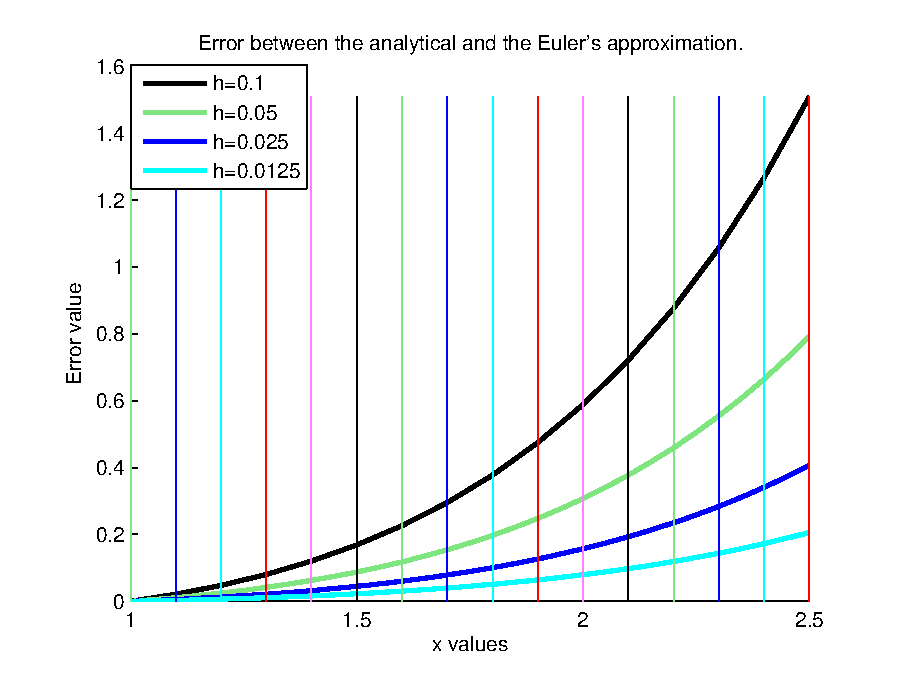
\includegraphics[width=2.5in]{rsrc/example.eps}
\caption{Simulation Results}
\label{fig_sim}
\end{figure}
\section {Methods}
\subsection{Normalization}
Preprocessing of the image is needed in order to have a good recognition. We'll use for this purpose equalized gray images. The first thing is to detect the face. We use Haar features to detect it. However, Haar will only recognize not rotated face. If we do not recognize a face, the face will be rotated and the same process will be used. Once a face is detected we'll use again Haar features to detect the eyes or the mouth and nose. The angle remaining to have the eyes or nose and mouth aligned is then used to have these features aligned. The face is then cropped to the dimensions of the face detected by Haar features and resize to a specified size, so that every picture has the same size.


\subsection{Fisher method}
\begin{figure}
	\centering		
	\includegraphics[width = 0.4\textwidth]{rsrc/LDA_basic.png}
	\caption{Az LDA algoritmus által megvizsgált szórások. The source of the image: \cite{LDA}}
	\label{fig:LDA abrazolas}
\end{figure}

Ha $ m $ dimenziós vektorokat szeretnék leképezni egy $ C $-dimenziós térbe akkor azt a következő módon tehetem meg.
\begin{equation}
y = w^Tx \textrm{, where } 
\end{equation}
\begin{equation}
x = \left(
\begin{array}{ccc}
x_1\\
\vdots\\
x_m
\end{array} \right)
w=\left(
\begin{array}{ccc}
w_{1,1} \dots w_{1,C}\\
\vdots \ddots \vdots\\
w_{m,1} \dots w_{m,C}
\end{array}
\right)
y = \left(
\begin{array}{ccc}
y_1\\
\vdots\\
y_C
\end{array}\right)
\label{equ:Alap_egyenlet}
\end{equation}

\subsection{Eigenfaces method}

The Eigenfaces method is based on a principal components analysis from a training set of images. To get those, each normalized image is translated into a vector. The principal components will be then determined : They have the highest eigenvalue in the diagonalized correlation matrix (made out of the image and the mean values of the training set). After selecting the principals components (first eigenvectors called eigenfaces in this case), each image can be then be approximated with those weighed eigenfaces :
\begin{equation}
x \approx  \hat{x} = \bar{x} + E_{x} * W \textrm{, where } 
\end{equation}
$x$ = vector representing the image,\\
$\hat{x}$ = approximated vector,\\
$\bar{x}$ = mean values of the vector during training,\\
$E_{x}$ = Matrix of eigenfaces (principal components),\\
$W$ = Matrix of weights of eigenfaces\\

$W$ is particular to each image and is calculated to minimize the distance between $x$ and $\bar{x}$:
\begin{equation}
W = E_{x}^T (x-\bar{x}) 
\end{equation}

The face recognized will be then the one in the training having its weight matrix $W$ the closest to the weight matrix of the current face analyzed. 

\subsection{Local Binary Pattern Histogram}

The local binary pattern histogram method uses the local feature of the face. First, the image is sliced into squares.
To avoid problems of scale, The neighbours of a pixel analysed will be the ones on a circle with a varying radius and this pixel as center.
The intensity of the central pixel is then compared to the ones of its neighbours. (higher values become 1, lower ones become 0).
We then compute the new value of the central pixel, being the sum of powers of two combined with the value of neighbor taken clockwise. The point is to spot particular patterns of neighbor such as edges, lines, corner, flat areas.

\begin{figure}[ht]
\centering
\includegraphics[width=2.5in]{rsrc/LBPH1.jpg}
\caption{Analysing the local structure}
\label{Local Structure}
\end{figure}

The histograms are then added (and not merged) for each part of the image. The resulting vector is then compared to the vectors obtained during the training. A fixed number of the closest vectors to the resulting vector is chosen and the person assigned to the greater number of these vector will be associated with the initial image.

\begin{figure}[ht]
\centering
\includegraphics[width=2.5in]{rsrc/LBPH2.png}
\caption{Adding histograms (source : http://what-when-how.com/face-recognition/)}
\label{Adding histograms}
\end{figure}

\section {Implementation}
\subsection{The Graphical User Interface}

To make our program simple and easy to use, we have created a Graphical User Interface(GUI). To do so we have used the Qt library and because it can 
generate problems on some computers, the program can also be run without GUI by specifying the training and testing folders in the command line.
The GUI is divided into 3 main parts: the main window, the result dialogBox and the ImageCapture program.

\subsubsection{The main window}

It is the first window to appear when the program is executed. It contains the following functionalities:
\begin{itemize}
 \item A menu to load and save classifiers in a file (the classifier selected in the list of methods will be used) and to run the ImageCapture 
program.

\item A path selection tool to specify where is are the training and validation folders. The paths can be modified directly from the text inputs or 
by browsing it using the "..." button.

\item A widget displaying the image retrieved from the webcam. A Rectangle has been added to help the user to center his face on the picture.
\item An output console embedded in the window.
\item A normalization checkbox to apply the normalization on the images or not
\item A progressBar to make sure that the program is still running while loading the images (unfortunately it was not possible to do the same for the 
training).
\end{itemize}

\subsubsection{The result dialogBox}
When a new picture is taken by the user, a new result window is created. This dialogBox call the predict function from the selected classifier and 
display the results to the user(image, predicted label and confidence level).

\subsubsection{The ImageCapture program}
- Drag'n Drop square
- Big cross for alignment
- Space Bar to record

\subsubsection{The Webcam object}

\subsection{Dataset seperation}

We have broken down our initial dataset into 2 folders: a training folder and a testing one.


\section{Results}
We validated our implementations with our database. It's contains around 15 training and 200 testing pictures about each team member. In the test set in contains one more person (Andris) to test the result for an unknown face.

The average successful classification ratio.
\begin{itemize}
	\item Eigen face: 71.65\%
	\item Fisher face: 90.80\%
	\item LBPH: 86.81\%
\end{itemize}

The results for the combined classifier:
\begin{table}[h]
	\begin{tabular}{l|l}
		** Classification Rate:                ** &          \\ \hline
		Adrian                                    & 94.26\%  \\
		Axel                                      & 94.12\%  \\
		Carole                                    & 99.63\%  \\
		Domi                                      & 99.39\%  \\
		Gareth                                    & 100.00\% \\ \hline
		Full Result                               & 97.48\%  \\ 
		\\
		** Unsuccesful classification:         ** &          \\ \hline
		Adrian:                                   & 13.64\%  \\
		Axel:                                     & 36.57\%  \\
		Carole:                                   & 5.61\%   \\
		Domi:                                     & 25.23\%  \\
		Gareth:                                   & 0.69\%  \\ \hline
		Andris:                                   & 73.10\%  
	\end{tabular}
	\label{CombinedResult}
	\title{Combined classifier validation result}
\end{table}

The results shows that the combined classifier has 7\% better result than the fisher faces method. The reason is the usage of the boosting. We combined 3 independent method to achieve a better solution than any of it. An other important difference is that the Fisher and the eigenface method did not use threshold for the decision. Because of that if an unknown face would be tried to classify the method would return one of the known label in any circumstances. The combined classifier result shows that the unknown person (Andris) 73\% classified as not recognizable face.
\section{Conclusion}
Face Regnition is a complex and popular problem with a large domain of applications and a lot of methods have been developed since the 
2000's. During this project we have used the OpenCV FaceRecognition module to create different Recognizers. We have then developed a graphical user 
interface to train and test the recognizers easily but also to take pictures from the camera and to predict the name of the person in front of the 
it. We have finally created a database of our faces and tested the different methods with it and with official databases. We came to the 
following results. EigenFaces > FisherFaces > LBPH (to be detailed). But more interesting, if we combine the different classifiers and make a 
decision rule based on the result of each classifier we obtain a more robust recongizer.
\appendices

\section{Important code parts}
Appendix two text goes here.


\bibliographystyle{IEEEtran}
\bibliography{rsrc/bibliography} % adjust this to fit your BibTex file

% that's all folks
\end{document}


